\documentclass[]{article}
\newcommand{\FileDepth}{../../..}
\usepackage[letterpaper, landscape, margin=0.5cm]{geometry}
\usepackage[T1]{fontenc}
\usepackage{textcomp}%Not strictly necessary, but gives \textmu command for "micro."
\usepackage{fancyhdr}
\usepackage{amsmath}
\usepackage{amssymb}
\usepackage{graphicx}
\usepackage{xcolor}
\usepackage{tikz}
\usetikzlibrary{calc}
\usepackage[shortlabels]{enumitem}
\usepackage{multicol}
\usepackage{vwcol}
\usepackage{hyperref}
\usepackage{wrapfig}
%opening
\newcommand{\SecType}{S}
\newcommand{\Week}{6}
\title{PH 211 Studio \Week}
\author{Benjamin Bauml}
\date{Summer 2024}

\newcommand{\Purpose}{4}
\newcommand{\DefOnly}{0}

% Version 2024-06-14
% Changes
% 2024-02-21 Added xstring package to enable smooth implementation of new \ModePage command.
% 2024-04-27 Set up to split activities and formatting aspects into separate files. Removed dependence on xcomment. Added an automatic counter to number the activities in a problem set.
% 2024-05-19 Revised old format for \TeachingTips command, which did not support \DefOnly.
% 2024-06-14 Added Repurpose environment to allow mixing of different purpose levels in the same document.
\usepackage{tcolorbox}
\usepackage{xstring}
% You will want the following four lines in your document (the last two uncommented):
% For Assignment, leave Purpose as 1. For Worksheet, set to 2. For Student Solution, set to 3. For Teacher Solution, set to 4.
% If you want keep the pieces from being called manually, set DefOnly to 0.
%\newcommand{\Purpose}{4}
%\newcommand{\DefOnly}{1}
\newcommand{\Exclusion}{0}
\newcommand{\PageTurn}{0}
\newcommand{\GrayProb}{0}
\newcommand{\Tipsy}{0}

% Assignment
\if\Purpose1
\renewcommand{\Exclusion}{1}
\fi
% Worksheet
\if\Purpose2
\renewcommand{\Exclusion}{1}
\renewcommand{\PageTurn}{1}
\fi
% Student Solution
\if\Purpose3
\renewcommand{\PageTurn}{1}
\renewcommand{\GrayProb}{1}
\fi
% Teaching Copy
\if\Purpose4
\renewcommand{\PageTurn}{1}
\renewcommand{\GrayProb}{1}
\renewcommand{\Tipsy}{1}
\fi

\newenvironment{Repurpose}[1]{
\renewcommand{\Purpose}{#1}
\renewcommand{\Exclusion}{0}
\renewcommand{\PageTurn}{0}
\renewcommand{\GrayProb}{0}
\renewcommand{\Tipsy}{0}
% Assignment
\if\Purpose1
\renewcommand{\Exclusion}{1}
\fi
% Worksheet
\if\Purpose2
\renewcommand{\Exclusion}{1}
\renewcommand{\PageTurn}{1}
\fi
% Student Solution
\if\Purpose3
\renewcommand{\PageTurn}{1}
\renewcommand{\GrayProb}{1}
\fi
% Teaching Copy
\if\Purpose4
\renewcommand{\PageTurn}{1}
\renewcommand{\GrayProb}{1}
\renewcommand{\Tipsy}{1}
\fi
}{}

\def \NewQ {0}
\def \PForce {0}
\newcommand{\MaybePage}[1]{
	\def \PForce {#1}
	\if\PForce1
	\newpage
	\else
	\if\NewQ0
	\gdef \NewQ {\PageTurn}
	\else
	\newpage
	\fi
	\fi
}

\newcommand{\ModePage}[1]{
	\IfSubStr{#1}{\Purpose}{\newpage}{}
}

\newcounter{ActNumber}
\setcounter{ActNumber}{0}

\newcommand{\Problem}[4][0]{%The first argument is optional, and if it is set to 1, the \newpage will be forced. The second argument is the name of the activity, the third is the command the activity is stored as, and the fourth is the actual problem statement.
\newcommand{#3}{
\MaybePage{#1}
\addtocounter{ActNumber}{1}
\section*{\SecType\Week-\theActNumber: #2}
\if\GrayProb1
\begin{tcolorbox}[colback=lightgray,colframe=lightgray,sharp corners,boxsep=1pt,left=0pt,right=0pt,top=0pt,bottom=0pt,after skip=2pt]
\else
\begin{tcolorbox}[colback=white,colframe=white,sharp corners,boxsep=1pt,left=0pt,right=0pt,top=0pt,bottom=0pt,after skip=2pt]
\fi
#4
\end{tcolorbox}\noindent
}
\if\DefOnly0
\else
#3
\fi
}
	
\newcommand{\ProblemSub}[3][0]{%The first argument is optional, and if a string of numbers is entered into it, it will force a \newpage in any \Purpose that shows up in the string. For example, "13" would lead to the newpage being forced in modes 1 and 3. The second is the command the activity is stored as, and the third is the actual problem statement.
\newcommand{#2}{
\ModePage{#1}
\if\GrayProb1
\begin{tcolorbox}[colback=lightgray,colframe=lightgray,sharp corners,boxsep=1pt,left=0pt,right=0pt,top=0pt,bottom=0pt,after skip=2pt]
\else
\begin{tcolorbox}[colback=white,colframe=white,sharp corners,boxsep=1pt,left=0pt,right=0pt,top=0pt,bottom=0pt,after skip=2pt]
\fi
#3
\end{tcolorbox}\noindent
}
\if\DefOnly0
\else
#2
\fi
}
		
\newcommand{\Solution}[2]{%The first argument is the command the solution is stored as, and the second is the actual solution.
\newcommand{#1}{
\if\Exclusion0
#2
\fi
}
\if\DefOnly0
\else
#1
\fi
}
		
\newcommand{\ProblemFig}[2]{%The first argument is the command the figure is stored as, and the second is the actual figure.
\newcommand{#1}{
\begin{figure}[h]
#2
\end{figure}
}
\if\DefOnly0
\else
#1
\fi
}

\newcommand{\TeachingTips}[2]{%The first argument is the command the tip is stored as, and the second is the actual tip.
\newcommand{#1}{
\if\Tipsy1
\begin{tcolorbox}[colback=lightgray,colframe=black]
#2
\end{tcolorbox}
\fi
}
\if\DefOnly0
\else
#1
\fi
}
\usepackage[absolute]{textpos}
% This package relies on Assignment Format 2024-06-14 or later to work. It is recommended that the Purpose and DefOnly commands be given as such:
%\newcommand{\Purpose}{4}
%\newcommand{\DefOnly}{0}
% Activities need to be entered outside of the TeacherMargin and PresentSpace environments, otherwise they will be defined only locally. They can even go in the preamble.
\newenvironment{TeacherMargin}{\begin{textblock*}{10.8cm}(0.5cm,0.5cm)
\small}{\end{textblock*}
\hspace{0.1cm}}
\newenvironment{PresentSpace}{\begin{textblock*}{0.3cm}(26.85cm,9.35cm)
--
\end{textblock*}
\begin{textblock*}{0.3cm}(26.85cm,18.7cm)
--
\end{textblock*}
\begin{textblock*}{0.3cm}(26.85cm,12.24cm)
	--
\end{textblock*}
\begin{textblock*}{15.6cm}(11.8cm,0.5cm)
\begin{Repurpose}{1}
\Large}{\end{Repurpose}
\end{textblock*}
\hspace{0.1cm}}

\newcommand{\FBDaxes}[3]{
	\begin{scope}[shift={(#1)},rotate=#2]
		% x-axis
		\draw[thick,->] (-2,0) -- (2,0);
		\node[anchor=west] at (2,0) {$x$};
		% y-axis
		\draw[thick,->] (0,-2) -- (0,2);
		\node[anchor=west] at (0,2) {$y$};
		\coordinate (#3) at (0,0);
	\end{scope}
}
\newcommand{\FBDvectorMA}[4]{
	\begin{scope}[shift={(#1)}]
		\coordinate (#4tip) at ({#2*cos(#3)},{#2*sin(#3)});
		\draw[ultra thick,blue,->] (#1) -- (#4tip);
	\end{scope}
}
\newcommand{\FBDvectorXY}[3]{
	\begin{scope}[shift={(#1)}]
		\coordinate (#3tip) at (#2);
		\draw[ultra thick,blue,->] (0,0) -- (#3tip);
	\end{scope}
}
\newcommand{\FBDdot}[1]{
	\filldraw[black] (#1) circle (3pt);
}
%\newcommand{\MVec}[3][0]{%Creates a momentum vector of length #3 centered at #2 and rotated #1 degrees counterclockwise.
	\begin{scope}[rotate=#1,shift={(#2)}]
		\draw[->,thick] ({-#3/2},0) -- ({#3/2},0);
	\end{scope}
}
\newcommand{\MDot}[1]{%Creates a dot at #1 to represent a zero vector.
	\filldraw (#1) circle (1pt);
}
\newcommand{\MVDRows}[2][4.5]{%Creates the rows (initial, delta, final) of a momentum vector diagram. The optional argument determines the width of the table, and defaults to a good length for three columns (two objects and the total system). The non-optional argument gives a coordinate name (not displayed) to the diagram.
	\begin{scope}
		%\draw[thick] (0,5.5) -- (0,0);
		\draw[thick] (-1,4.5) -- (#1,4.5);
		\node at (-0.5,3.75) {$\vec{p}_{i}$};
		\draw[thick] (-1,3) -- (#1,3);
		\node at (-0.5,2.25) {$\Delta\vec{p}$};
		\draw[thick] (-1,1.5) -- (#1,1.5);
		\node at (-0.5,0.75) {$\vec{p}_{f}$};
		\coordinate (#2) at (0,5);
	\end{scope}
}
\newcommand{\MVDCol}[4][0.75]{%Creates a column for an object in a momentum vector diagram. The first (non-optional) argument is the coordinate name (not displayed) of the column, while the second is the displayed column header. The first argument also names the three entries down the column. The third argument anchors the column, so it should either be the coordinate name of the MVD (for the first column) or the coordinate name of the previous column. The optional argument indicates how far the center of the column should be from the previous column's edge, and defaults to 0.75
	\begin{scope}[shift={(#4)}]
		\node at (#1,0) {#3};
		%\draw[thick] ({#1*2},0.5) -- ({#1*2},-5);
		\draw[thick] (0,0.5) -- (0,-5);
		\coordinate (#2init) at (#1,-1.25);
		\coordinate (#2delt) at (#1,-2.75);
		\coordinate (#2fin) at (#1,-4.25);
		\coordinate (#2) at ({#1*2},0);
	\end{scope}
}

%\input{\FileDepth/Activities/Activity_One/Activity_One.tex}
%\input{\FileDepth/Activities/Activity_Two/Activity_Two.tex}

\begin{document}
\begin{TeacherMargin}
\noindent Since the force is constant in magnitude and direction, the work simplifies to
\[
W = \vec{F}_{0} \cdot \Delta\vec{s}.
\]
\textbf{Case 1} \\
$\vec{F}_{0}$ is parallel to $\Delta\vec{s}$, so $W_{1} = \vec{F}_{0} \cdot \Delta\vec{s} = F_{0}\Delta s > 0$. \\
\textbf{Case 2} \\
$\vec{F}_{0}$ makes an acute angle with $\Delta \vec{s}$ (let's call this angle, the angle $\Delta \vec{s}$ makes below the horizontal, $\theta$), so $W_{2} = \vec{F}_{0} \cdot \Delta\vec{s} = F_{0}\Delta s\cos\theta$, where $0<\cos\theta<1$, so $W_{2}>0$. \\
\textbf{Case 3} \\
$\vec{F}_{0}$ is perpendicular to $\Delta \vec{s}$ so $W_{3} = \vec{F}_{0} \cdot \Delta\vec{s} = 0$. \\
In this case, remember that the push from the hand and the motion of the block are not necessarily related. The block is already moving for some reason, and we choose to push down on it. We may push, and our hand may move with it, but we add no energy to the system by pushing in a direction the block isn't moving. \\

\noindent Since all of the works are nonnegative, they are equal to their absolute values, and we can rank them as follows:
\[
W_{1} > W_{2} > W_{3} = 0.
\]
\end{TeacherMargin}
\begin{PresentSpace}
\begin{center}
	\huge Studio 6: Work and Kinetic Energy
\end{center}
\underline{Warm-Up Activity} \\
A block is moving to the right (displacement $\Delta\vec{s}$) while a hand exerts a force of magnitude $F_{0}$ on the block.
\begin{itemize}
	\item In each case, is the work done by the hand \textit{positive}, \textit{negative}, or \textit{zero}?
	\item How does the absolute value of the work compare in the three cases?
\end{itemize}
\begin{center}
	\begin{tikzpicture}
		\begin{scope}
			\draw[thick] (0,0) rectangle (4,4);
			\node[anchor=north west] at (0,4) {Case 1};
			\filldraw[lightgray] (0.3,1) rectangle (3.7,0.7);
			\draw[thick,lightgray,dashed] (0.5,1) rectangle (1.5,2);
			\draw[ultra thick] (0.3,1) -- (3.7,1);
			\draw[ultra thick,->] (0.5,0.7) -- (1.5,0.7) node[anchor=north] {$\Delta\vec{s}$} -- (2.5,0.7);
			\draw[thick] (2.5,1) rectangle (3.5,2);
			\draw[ultra thick,->,shift={(2.5,1.7)}] (0,0) -- (0.7,0);
			\node[rotate=-60] at (2.53,2.3) {
\includegraphics[scale=1.3]{KnightHand}};
		\end{scope}
		\begin{scope}[shift={(4.5,0)}]
			\draw[thick] (0,0) rectangle (4,4);
			\node[anchor=north west] at (0,4) {Case 2};
			\filldraw[lightgray] (0.3,1) rectangle (3.7,0.7);
			\draw[thick,lightgray,dashed] (0.5,1) rectangle (1.5,2);
			\draw[ultra thick] (0.3,1) -- (3.7,1);
			\draw[ultra thick,->] (0.5,0.7) -- (1.5,0.7) node[anchor=north] {$\Delta\vec{s}$} -- (2.5,0.7);
			\draw[thick] (2.5,1) rectangle (3.5,2);
			\draw[ultra thick,->,shift={(2.5,1.9)},rotate=-30] (0,0) -- (0.7,0);
			\node[rotate=-70] at (2.65,2.4) {
\includegraphics[scale=1.3]{KnightHand}};
		\end{scope}
		\begin{scope}[shift={(9,0)}]
			\draw[thick] (0,0) rectangle (4,4);
			\node[anchor=north west] at (0,4) {Case 3};
			\filldraw[lightgray] (0.3,1) rectangle (3.7,0.7);
			\draw[thick,lightgray,dashed] (0.5,1) rectangle (1.5,2);
			\draw[ultra thick] (0.3,1) -- (3.7,1);
			\draw[ultra thick,->] (0.5,0.7) -- (1.5,0.7) node[anchor=north] {$\Delta\vec{s}$} -- (2.5,0.7);
			\draw[thick] (2.5,1) rectangle (3.5,2);
			\draw[ultra thick,->,shift={(3,2)}] (0,0) -- (0,-0.7);
			\node[rotate=-60] at (3.1,2.8) {
\includegraphics[scale=1.3]{KnightHand}};
		\end{scope}
	\end{tikzpicture}
\end{center}
\end{PresentSpace}
\newpage
\begin{TeacherMargin}

\end{TeacherMargin}
\begin{PresentSpace}
\vspace{-10pt}
\section*{A Deeper Model for Interactions}
\vspace{-10pt}
\begin{itemize}
	\item Quantities
	\begin{itemize}
		\item Energy \qquad \qquad \qquad \quad \ \ $E$
		\item Work \qquad \qquad \qquad \quad \ \ \ $W = \int_{r_{i}}^{r_{f}}\vec{F}\cdot d\vec{r}$
		\item Kinetic Energy \qquad \qquad $K=\frac{1}{2}mv^{2}$
	\end{itemize}
	\item Laws
	\begin{itemize}
		\item Work-energy theorem \quad $W_{\text{net,ext}} = \Delta E_{\text{total}}$
	\end{itemize}
\end{itemize}
\end{PresentSpace}
\newpage
\begin{TeacherMargin}
\noindent The free body diagram is the same in both stages:
\begin{center}
	\begin{tikzpicture}
		\FBDbox{0,0}{0}{block}{}
		\FBDvectorXY{blocktcent}{0,1}{FNS}
		\node[anchor=east] at (FNStip) {$\vec{F}^{N}_{BS}$};
		\FBDvectorXY{blocklcent}{-1,0}{FNH}
		\node[anchor=east] at (FNHtip) {$\vec{F}^{N}_{BH}$};
		\FBDvectorXY{blockbcent}{0,-1}{FG}
		\node[anchor=east] at (FGtip) {$\vec{F}^{g}_{BE}$};
	\end{tikzpicture}
\end{center}
The work done by the normal force from the surface and work done by the force of gravity are both zero, as these forces are perpendicular to the horizontal displacement. For the force from the hand, let us fill in the table (for two different choices of coordinate system):
\begin{center}
	\normalsize
	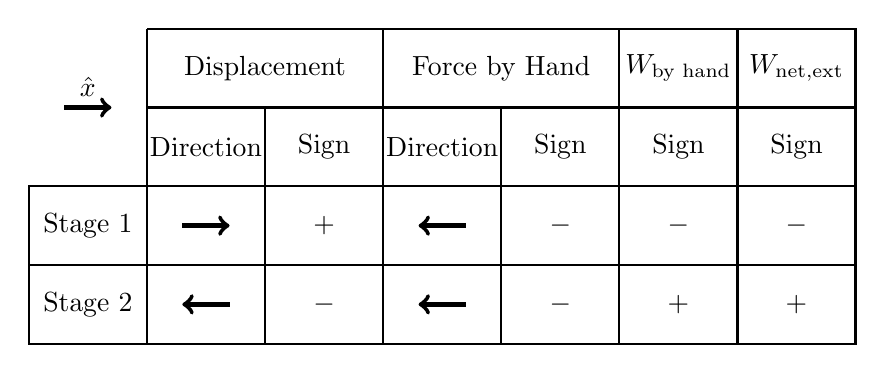
\begin{tikzpicture}
		\draw[ultra thick,->,shift={(-0.75,3)}] (-0.3,0) -- (0,0) node [anchor=south] {$\hat{x}$} -- (0.3,0);
		\draw[thick] (0,2) -- (-1.5,2) -- (-1.5,0) -- (9,0) -- (9,4) -- (0,4);
		\draw[thick] (0,3) -- (9,3);
		\draw[thick] (7.5,3) -- (7.5,4);
		\draw[thick] (0,2) -- (9,2);
		\draw[thick] (-1.5,1) -- (9,1);
		\foreach \x in {0,1,2}
		\draw[thick] (3*\x,0) -- (3*\x,4);
		\foreach \x in {0,1,2}
		\draw[thick] (3*\x+1.5,0) -- (3*\x+1.5,3);
		\foreach \y in {1,2}
		\node at (-0.75,2.5-\y) {Stage \y};
		\foreach \x in {0.75,3.75}
		\node at (\x,2.5) {Direction};
		\foreach \x in {2.25,5.25,6.75,8.25}
		\node at (\x,2.5) {Sign};
		\node at (1.5,3.5) {Displacement};
		\node at (4.5,3.5) {Force by Hand};
		\node at (6.75,3.5) {$W_{\text{by hand}}$};
		\node at (8.25,3.5) {$W_{\text{net,ext}}$};
		\draw[ultra thick,->,shift={(0.75,1.5)}] (-0.3,0) -- (0.3,0);
		\draw[ultra thick,<-,shift={(0.75,0.5)}] (-0.3,0) -- (0.3,0);
		\node at (2.25,1.5) {$+$};
		\node at (2.25,0.5) {$-$};
		\draw[ultra thick,<-,shift={(3.75,1.5)}] (-0.3,0) -- (0.3,0);
		\draw[ultra thick,<-,shift={(3.75,0.5)}] (-0.3,0) -- (0.3,0);
		\node at (5.25,1.5) {$-$};
		\node at (5.25,0.5) {$-$};
		\node at (6.75,1.5) {$-$};
		\node at (6.75,0.5) {$+$};
		\node at (8.25,1.5) {$-$};
		\node at (8.25,0.5) {$+$};
	\end{tikzpicture}
\end{center}
\begin{center}
	\normalsize
	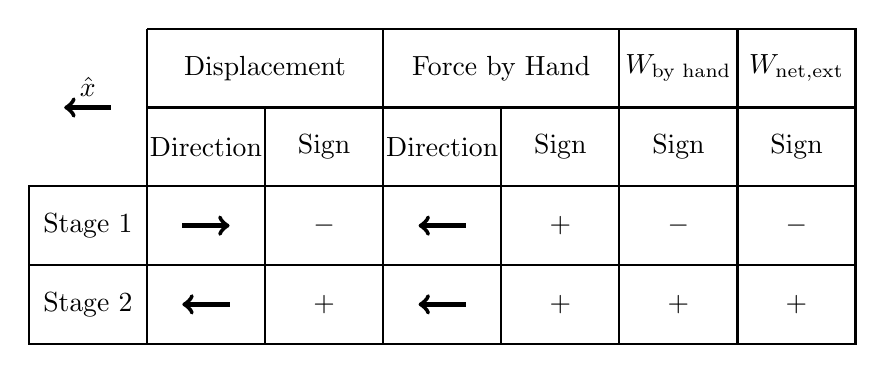
\begin{tikzpicture}
		\draw[ultra thick,<-,shift={(-0.75,3)}] (-0.3,0) -- (0,0) node [anchor=south] {$\hat{x}$} -- (0.3,0);
		\draw[thick] (0,2) -- (-1.5,2) -- (-1.5,0) -- (9,0) -- (9,4) -- (0,4);
		\draw[thick] (0,3) -- (9,3);
		\draw[thick] (7.5,3) -- (7.5,4);
		\draw[thick] (0,2) -- (9,2);
		\draw[thick] (-1.5,1) -- (9,1);
		\foreach \x in {0,1,2}
		\draw[thick] (3*\x,0) -- (3*\x,4);
		\foreach \x in {0,1,2}
		\draw[thick] (3*\x+1.5,0) -- (3*\x+1.5,3);
		\foreach \y in {1,2}
		\node at (-0.75,2.5-\y) {Stage \y};
		\foreach \x in {0.75,3.75}
		\node at (\x,2.5) {Direction};
		\foreach \x in {2.25,5.25,6.75,8.25}
		\node at (\x,2.5) {Sign};
		\node at (1.5,3.5) {Displacement};
		\node at (4.5,3.5) {Force by Hand};
		\node at (6.75,3.5) {$W_{\text{by hand}}$};
		\node at (8.25,3.5) {$W_{\text{net,ext}}$};
		\draw[ultra thick,->,shift={(0.75,1.5)}] (-0.3,0) -- (0.3,0);
		\draw[ultra thick,<-,shift={(0.75,0.5)}] (-0.3,0) -- (0.3,0);
		\node at (2.25,1.5) {$-$};
		\node at (2.25,0.5) {$+$};
		\draw[ultra thick,<-,shift={(3.75,1.5)}] (-0.3,0) -- (0.3,0);
		\draw[ultra thick,<-,shift={(3.75,0.5)}] (-0.3,0) -- (0.3,0);
		\node at (5.25,1.5) {$+$};
		\node at (5.25,0.5) {$+$};
		\node at (6.75,1.5) {$-$};
		\node at (6.75,0.5) {$+$};
		\node at (8.25,1.5) {$-$};
		\node at (8.25,0.5) {$+$};
	\end{tikzpicture}
\end{center}
The work done by a force does not depend on your choice of coordinate system. There are some signs that are coordinate system dependent (such as those applied to the directions of vectors), but those with physical meaning (such as the sign of work, which indicates whether energy is entering or leaving the system) do not. \\

\noindent The work done is negative in stage 1, where the force is opposite the displacement. Energy is subtracted from the system, and the speed of the block decreases. \\

\noindent The work done is positive in stage 2, where the force is in the same direction as the displacement. Energy is added to the system, and the speed of the block increases.
\end{TeacherMargin}
\begin{PresentSpace}
\vspace{-10pt}
\section*{S6-1: Reversing a Block}
\vspace{-10pt}
\begin{itemize}
	\item A block is initially moving to the right on a level, frictionless surface. The system consists of only the block.
	\item A hand exerts a constant horizontal force on the block that causes the block to slow down (stage 1), then move in the opposite direction while speeding up (stage 2).
	\item For each stage:
	\begin{itemize}
		\item Draw a free-body \\
		diagram for the \\
		block.
		\item Determine \\
		whether the \\
		work done by each force is positive, negative, or zero.
		\item Fill in the table:
	\end{itemize}
\end{itemize}
\end{PresentSpace}
\begin{textblock*}{10cm}(17cm,4.75cm)
	\begin{center}
		\normalsize
		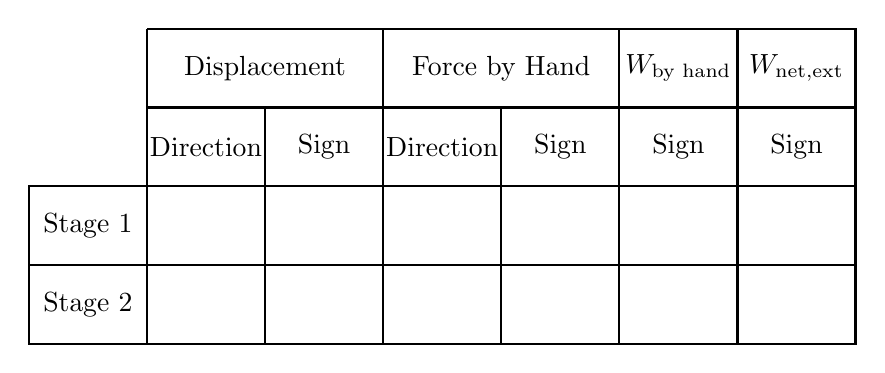
\begin{tikzpicture}
			\draw[thick] (0,2) -- (-1.5,2) -- (-1.5,0) -- (9,0) -- (9,4) -- (0,4);
			\draw[thick] (0,3) -- (9,3);
			\draw[thick] (7.5,3) -- (7.5,4);
			\draw[thick] (0,2) -- (9,2);
			\draw[thick] (-1.5,1) -- (9,1);
			\foreach \x in {0,1,2}
			\draw[thick] (3*\x,0) -- (3*\x,4);
			\foreach \x in {0,1,2}
			\draw[thick] (3*\x+1.5,0) -- (3*\x+1.5,3);
			\foreach \y in {1,2}
			\node at (-0.75,2.5-\y) {Stage \y};
			\foreach \x in {0.75,3.75}
			\node at (\x,2.5) {Direction};
			\foreach \x in {2.25,5.25,6.75,8.25}
			\node at (\x,2.5) {Sign};
			\node at (1.5,3.5) {Displacement};
			\node at (4.5,3.5) {Force by Hand};
			\node at (6.75,3.5) {$W_{\text{by hand}}$};
			\node at (8.25,3.5) {$W_{\text{net,ext}}$};
		\end{tikzpicture}
	\end{center}
\end{textblock*}
\newpage
\begin{TeacherMargin}
\noindent Pushed inward by the two forces, both blocks will accelerate, so they each have a nonzero final speed. They began at rest, so $K_{i} = 0$ J, and their final kinetic energy is $K_{f} = \frac{1}{2}m_{A}v_{A}^{2} + \frac{1}{2}m_{B}v_{B}^{2}$, there fore the change in kinetic energy of the system is positive ($\Delta K > 0$). \\

\noindent The force of the hand on A points right, and its point of application (where the hand is touching the block) is displaced to the right, so the work done by the hand is positive ($W_{A}^{\text{hand}}>0$). \\
For block B, the force of the hand and the displacement are both to the left, so the work is still positive ($W_{B}^{\text{hand}}>0$). \\
Note that $W_{B}^{\text{hand}}$ is not negative due to being ``in the opposite direction.'' The sign of work is determined by the direction of the force relative to the direction of the dipslacment of its point of contact. \\

\noindent The work done by gravity and the work done by the normal force on both blocks are zero ($W_{A}^{g} = W_{B}^{g} = W_{A}^{N} = W_{B}^{N}=0$). Their points of contact are displacing, but the forces are perpendicular to the displacement. \\

\noindent The net work is the sum of the individual works:
\begin{align*}
	W_{AB}^{\text{net}} & = W_{A}^{\text{net}} + W_{B}^{\text{net}} \\
	& = W_{A}^{\text{hand}} + W_{A}^{g} + W_{A}^{N} + W_{B}^{\text{hand}} + W_{B}^{g} + W_{B}^{N} \\
	& = W_{A}^{\text{hand}} + W_{B}^{\text{hand}} \\
	& > 0.
\end{align*}
The net work on the system is positive. \\
Note that the net work is \textbf{not} generally equal to the integral of the net force dotted with the displacement of the center of mass:
\[
W^{\text{net}} \neq \int\vec{F}^{net}\cdot d\vec{s}_{CoM}.
\]
This would give the wrong answer here, as the net force on AB is zero and the center of mass doesn't move. \\

\noindent Since both $W_{AB}^{\text{net}}>0$ and $\Delta K > 0$, our results are consistent with the work-energy theorem. Positive work increases the total energy of the system.
\end{TeacherMargin}
\begin{PresentSpace}
\vspace{-10pt}
\section*{S6-2: Pushing Boxes Together}
\vspace{-10pt}
Two identical blocks, A and B, are initially at rest on a level, frictionless surface. System AB consists of \textbf{both blocks}. \\
At time $t=t_{1}$, hands begin to push the blocks toward each other. \\
Each hand exerts a constant horizontal force of magnitude $F_{0}$. \\
At time $t=t_{2}$, each block has moved a distance $d_{0}$ from its initial position.
\begin{enumerate}[(1)]
	\large
	\item Determine if the \textbf{change in kinetic energy} of system AB is \textit{positive}, \textit{negative}, or \textit{zero}.
	\item Determine if the work done by \textbf{each force} is \textit{positive}, \textit{negative}, or \textit{zero}.
	\item Determine if the \textbf{net work} on system AB is \textit{positive}, \textit{negative}, or \textit{zero}.
	\item Check to see if your answers are consistent with the work-energy theorem.
\end{enumerate}
\begin{comment}
	\item Two identical blocks, A and B, are initially at rest on a level, frictionless surface. System AB consists of \textbf{both blocks}.
	\item At time $t=t_{1}$, hands begin to push the blocks toward each other as shown at right.
	\item Each hand exerts a constant horizontal force of magnitude $F_{0}$.
	\item At time $t=t_{2}$, each block has moved a distance $d_{0}$ from its initial position.
	\begin{enumerate}[(1)]
		\item Determine if the \textbf{change in kinetic energy} of system AB is \textit{positive}, \textit{negative}, or \textit{zero}.
		\item Determine if the work done by \textbf{each force} is \textit{positive}, \textit{negative}, or \textit{zero}.
		\item Determine if the \textbf{net work} on system AB is \textit{positive}, \textit{negative}, or \textit{zero}.
		\item Check to see if your answers are consistent with the work-energy theorem.
	\end{enumerate}
\end{comment}
\begin{center}
	\begin{tikzpicture}
		\node at (10,-2) {\parbox{3.5cm}{\centering Each hand pushes with a constant force of magnitude $F_{0}$.}};
		\begin{scope}
			\filldraw[lightgray] (0,0) rectangle (10,-0.5);
			\draw[ultra thick] (0,0) -- (10,0);
			\node[anchor=south west] at (0,0) {$t=t_{1}$};
			\node[rotate=-60] at (2.05,1.4) {
\includegraphics[scale=1.3]{KnightHand}};
			\draw[thick] (2,0) rectangle (3,1);
			\node at (2.5,0.5) {A};
			\node[yscale=-1,rotate=120] at (7.95,1.4) {
\includegraphics[scale=1.3]{KnightHand}};
			\draw[thick] (7,0) rectangle (8,1);
			\node at (7.5,0.5) {B};
			\draw[ultra thick,<->] (3,-0.5) -- (3.75,-0.5) node[anchor=north] {$d_{0}$} -- (4.5,-0.5);
			\draw[ultra thick,<->] (7,-0.5) -- (6.25,-0.5) node[anchor=north] {$d_{0}$} -- (5.5,-0.5);
		\end{scope}
		\begin{scope}[shift={(0,-3.5)}]
			\filldraw[lightgray] (0,0) rectangle (10,-0.5);
			\draw[ultra thick] (0,0) -- (10,0);
			\node[anchor=south west] at (0,0) {$t=t_{2}$};
			\node[rotate=-60] at (3.55,1.4) {
\includegraphics[scale=1.3]{KnightHand}};
			\draw[thick] (3.5,0) rectangle (4.5,1);
			\node at (4,0.5) {A};
			\node[yscale=-1,rotate=120] at (6.45,1.4) {
\includegraphics[scale=1.3]{KnightHand}};
			\draw[thick] (5.5,0) rectangle (6.5,1);
			\node at (6,0.5) {B};
			\draw[ultra thick,<->] (3,-0.5) -- (3.75,-0.5) node[anchor=north] {$d_{0}$} -- (4.5,-0.5);
			\draw[ultra thick,<->] (7,-0.5) -- (6.25,-0.5) node[anchor=north] {$d_{0}$} -- (5.5,-0.5);
		\end{scope}
	\end{tikzpicture}
\end{center}
\end{PresentSpace}
\newpage
\begin{TeacherMargin}
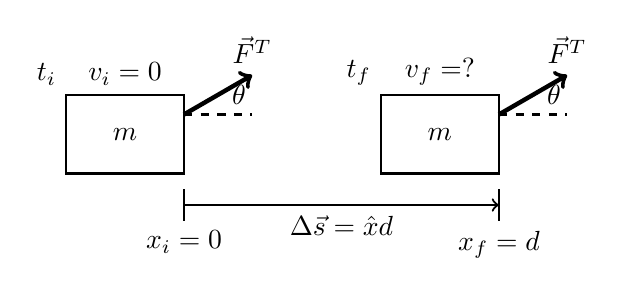
\begin{tikzpicture}
	\begin{scope}
		\draw[thick] (0,0) rectangle (1.5,1);
		\node[anchor=south east] at (0,1) {$t_{i}$};
		\node at (0.75,0.5) {$m$};
		\node[anchor=south] at (0.75,1) {$v_{i}=0$};
		\draw[ultra thick,->,shift={(1.5,0.75)},rotate=30] (0,0) -- (1,0) node[anchor=south] {$\vec{F}^{T}$};
		\draw[thick,dashed,shift={(1.5,0.75)}] (0,0) -- ({cos(30)},0);
		\node[anchor=south] at (2.2,0.75) {$\theta$};
		\draw[thick] (1.5,-0.2) -- (1.5,-0.6) node[anchor=north] {$x_{i}=0$};
	\end{scope}
	\begin{scope}[shift={(4,0)}]
		\draw[thick] (0,0) rectangle (1.5,1);
		\node[anchor=south east] at (0,1) {$t_{f}$};
		\node at (0.75,0.5) {$m$};
		\node[anchor=south] at (0.75,1) {$v_{f}=$?};
		\draw[ultra thick,->,shift={(1.5,0.75)},rotate=30] (0,0) -- (1,0) node[anchor=south] {$\vec{F}^{T}$};
		\draw[thick,dashed,shift={(1.5,0.75)}] (0,0) -- ({cos(30)},0);
		\node[anchor=south] at (2.2,0.75) {$\theta$};
		\draw[thick] (1.5,-0.2) -- (1.5,-0.6) node[anchor=north] {$x_{f}=d$};
	\end{scope}
	\draw[thick,->] (1.5,-0.4) -- (3.5,-0.4) node[anchor=north] {$\Delta \vec{s} = \hat{x}d$} -- (5.5,-0.4);
\end{tikzpicture}
Gravity and the normal force do no work here, so in general, for a force with constant direction:
\[
W^{net} = W^{T} = \int_{0}^{d}\vec{F}^{T}\cdot d\vec{x} = \int_{0}^{d}F^{T}\cos\theta dx = \cos\theta\int_{0}^{d}F^{T}dx.
\]
By the work-energy theorem, $W^{net}=\Delta K$, and since we know $K_{i} = 0$ and $K_{f}=\frac{1}{2}mv_{f}^{2}$, this means $v_{f} = \sqrt{\frac{2W^{net}}{m}}$. \\

\noindent\textbf{Case A} \\
For $F^{T} = T_{0}$, we have
\begin{align*}
	W_{T} & = T_{0}\cos\theta\int_{0}^{d}dx = T_{0}d\cos\theta, & v_{f} & = \sqrt{2\frac{T_{0}d}{m}\cos\theta}.
\end{align*}
\textbf{Case B} \\
To get a linear decrease (with respect to $x$) as described, the following equation should be used for the force:
\[
F^{T}(x) = 3T_{0}-\frac{2T_{0}}{d}x.
\]
This gives us
\begin{align*}
	W_{T} & = T_{0}\cos\theta\int_{0}^{d}\left(3-\frac{2}{d}x\right)dx \\
	& = T_{0}\cos\theta\left[3x-\frac{1}{d}x^{2}\right]_{x=0}^{d} \\
	& = T_{0}\cos\theta\left(3d-\frac{1}{d}d^{2}\right) \\
	& = 2T_{0}d\cos\theta, \\
	v_{f} & = 2\sqrt{\frac{T_{0}d}{m}\cos\theta}.
\end{align*}
\textbf{Unit Check} \\
2 and $\cos\theta$ are unitless, and as for the rest,
\[
\left[\sqrt{\frac{T_{0}d}{m}}\right] = \sqrt{\frac{[T_{0}][d]}{[m]}} = \sqrt{\frac{\text{kg}\cdot\text{m}\cdot\text{s}^{-2}\cdot\text{m}}{\text{kg}}} = \sqrt{\frac{\text{m}^{2}}{\text{s}^{2}}} = \frac{\text{m}}{\text{s}} = [v_{f}].
\]
\textbf{Covariation} \\
Pushing the block harder or pulling it farther will impart more kinetic energy, causing it to end up going faster. This is reflected in our equations, as increasing $T_{0}$ or $d$ causes $v_{f}$ to increase. \\
Pulling at a larger angle to the displacement is less efficient for doing work, and a more massive object resists accelerating more. This is reflected in our equations, as increasing $\theta$ or $m$ causes $v_{f}$ to decrease.
\end{TeacherMargin}
\begin{PresentSpace}
\vspace{-10pt}
\section*{S6-3: Dragging a Box}
\vspace{-10pt}
\begin{itemize}
	\item You are pulling a box with known mass $m$ at the angle shown below. The box moves from $x=0$ to $x=d$. Find the work done by the rope in each of the following situations:
	\begin{enumerate}[(A)]
		\item The tension is constant.
		\item The tension decreases linearly from $3T_{0}$ to $T_{0}$.
	\end{enumerate}
	\item If the box began at rest, find the \\
	final speed of the box in each of \\
	the situations above.
	\item Don't forget to make sense of \\
	your answers!
\end{itemize}
\end{PresentSpace}
\begin{textblock*}{10cm}(19cm,6cm)
\begin{center}
	\normalsize
	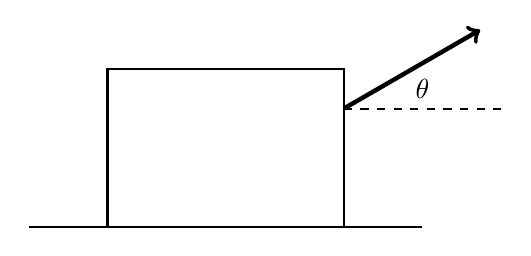
\begin{tikzpicture}
		\draw[thick] (0,0) rectangle (3,2);
		\draw[thick] (-1,0) -- (4,0);
		\draw[ultra thick,->,shift={(3,1.5)},rotate=30] (0,0) -- (2,0);
		\draw[thick,dashed] (3,1.5) -- (5,1.5);
		\node[anchor=south] at (4,1.5) {$\theta$};
	\end{tikzpicture}
\end{center}
\end{textblock*}
\newpage
\begin{TeacherMargin}

\end{TeacherMargin}
\begin{PresentSpace}
\section*{Main Ideas}
\begin{itemize}
	\item Energy is a powerful, ubiquitous concept that can help us solve a wide array of physics problems.
	\item Energy is a \textit{scalar}---it is not a vector.
	\item There are different forms of energy, and energy can be transferred between objects and between forms.
\end{itemize}
\end{PresentSpace}
\end{document}